\chapter{Requirements}
\section{Allgemeine Beschreibung}
\subsection{Produktperspektive}
Mit Internet of Things sind eine Vielzahl neuartige Devices entstanden. Während in herkömmlichen Netzwerken hauptsächlich Personal Computer, Notebooks, Server usw. verwaltet werden mussten, so bringen IoT Devices den IT-Abteilungen neue Herausforderungen. Zum einen dürfte die Anzahl Geräte gegenüber herkömmlichen Computer deutlich ansteigen, zum anderen sind IoT Devices in Sachen Funktionalität und Rechenleistung, sowie auch der Netzwerkbandbreite deutlich beschränkt. 

Mit <insert Application Name here> soll eine Management Applikation bereitgestellt werden, um eine Vielzahl unterschiedlicher IoT Devices administrieren zu können. 
\subsection{Produkfunktionen}
<insert Application Name here> soll den Benutzern erlauben, IoT Geräte zu verwalten. Die Aufgaben reichen vom Erfassen und Discovery von Devices über die Konfigurationsverwaltung und Softwareverteilung bis zu Backup und Restore. Ausserdem sollen Management-relevante Kommandos auf Devices ausgeführt- und Security Aspekte beachtet werden. Die Details zu den Produktfunktionen sind den Use Cases zu entnehmen.

\subsection{Benutzer Charakteristik}
Zielpersonen der Applikation sind Betreiber von IoT Devices. Dies können im Enterprise Umfeld IT-Mitarbeiter in operationeller Funktion-, oder auch Softwareentwickler für IoT Applikationen sein. Heimanwender können bei entsprechenden Kenntnissen ebenfalls zur Zielgruppe gehören. Es werden solide Grundkenntnisse in TCP/IP Netzwerken sowie Verständnis der verwendeten IoT Architekturen und Devices vorausgesetzt. 
\subsection{Einschränkungen}
Evtl. Browser Einschränkungen und bestimmte Use Cases, müsste nach Prototyp nochmals definiert werden
\section{Use Cases}
\subsection{Use Cases Diagramm}
\begin{figure}[H]
\centering
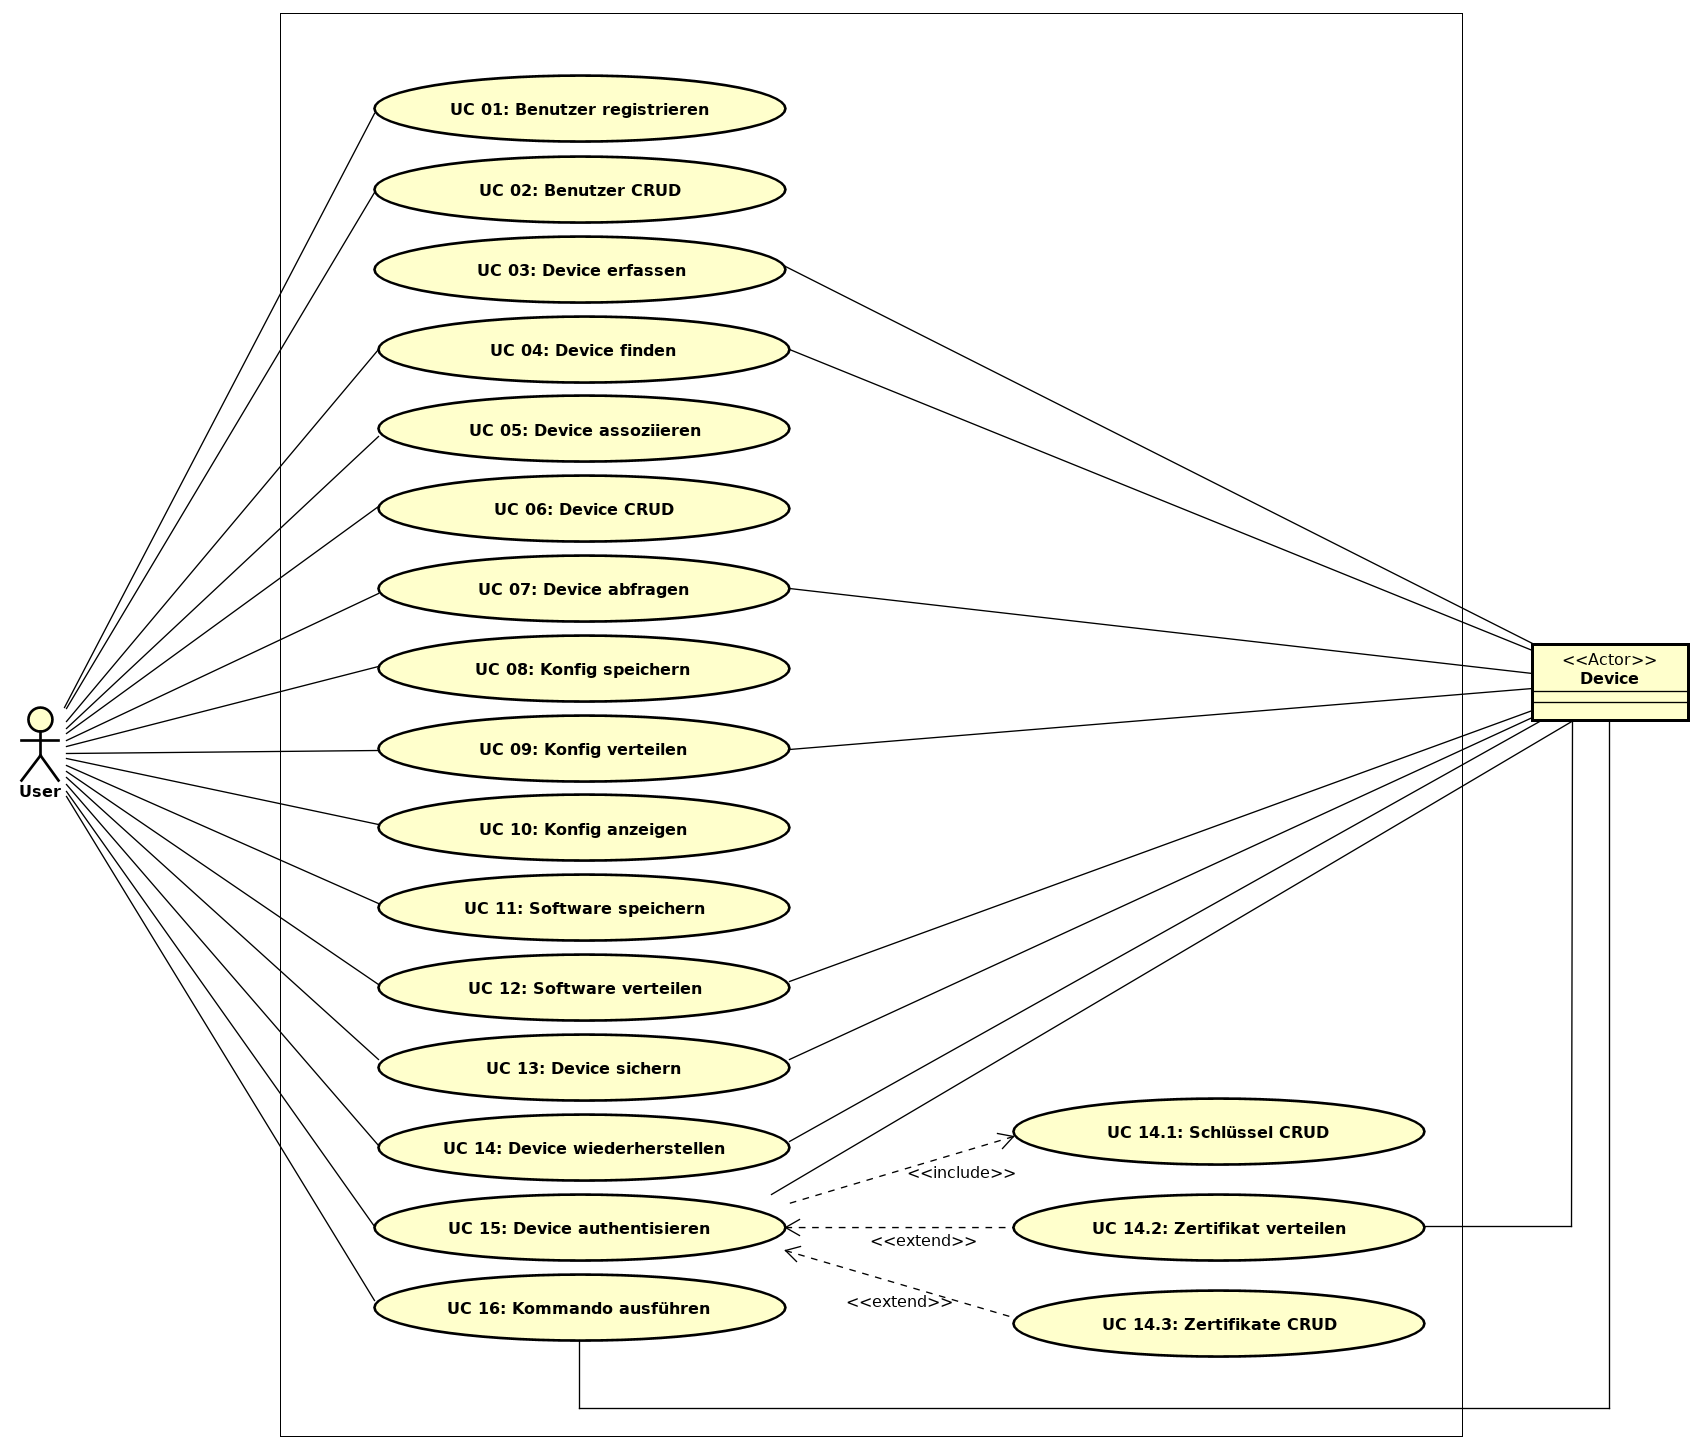
\includegraphics[scale=0.425]{images/use_case_diagram.png}\caption{Use Case Diagramm}
\end{figure}
\subsection{Aktoren}
Der Benutzer der Applikation ist in diesem System der einzige primäre Aktor.
\newpage
\subsection{Beschreibungen (Casual)}
\subsubsection{Benutzer CRUD}
\mbox{}
\begin{longtable}{| p{4cm} | p{11.7cm} |}
 \hline
 \textbf{ID} & 01\\ \hline 
 \textbf{Name} & Benutzer CRUD\\ \hline 
 \textbf{Beschreibung} & Benutzerverwaltung der Applikation\\ \hline 
 \textbf{Preconditions} & 
  \tabitem Applikation gestartet \newline
  \tabitem Benutzer ist registriert \newline
  \tabitem Benutzer ist eingeloggt \\ \hline 
 \textbf{Postconditions} & 
 \tabitem Änderungen gespeichert
 \\ \hline
 \textbf{Main Success Scenario} &
 \textbf{Create:}\newline
  1. UC 01: Benutzer registrieren \newline
 \textbf{Read:}\newline
  1. Benutzer lässt Userdaten anzeigen \newline
 \textbf{Update:}\newline
  1. Benutzer lässt Userdaten anzeigen \newline
  2. Benutzer verändert Attribute\newline
  3. Benutzer speichert Änderungen\newline
 \textbf{Delete:}\newline
  1. Benutzer wird gelöscht \\ 
 \hline 
 \textbf{Extensions} & -\\ \hline 
 \end{longtable}

\subsubsection{Device erfassen}
\mbox{}
\begin{longtable}{| p{4cm} | p{11.7cm} |}
 \hline
 \textbf{ID} & 02\\ \hline 
 \textbf{Name} & Device erfassen \\ \hline 
 \textbf{Beschreibung} & Der Benutzer möchte ein IoT Device finden. Entsprechende IoT Devices sollen dem Benutzer zur Adoption aufgelistet werden. \\ \hline 
 \textbf{Preconditions} & • \\ \hline 
 \textbf{Postconditions} & • \\ \hline 
 \textbf{Main Success Scenario} & • \\ \hline 
 \textbf{Extensions} & • \\ \hline 
\end{longtable}

\subsubsection{Device finden}
\mbox{}
\begin{longtable}{| p{4cm} | p{11.7cm} |}
 \hline
 \textbf{ID} & 03\\ \hline 
 \textbf{Name} & Device finden\\ \hline 
 \textbf{Beschreibung} & Der Benutzer möchte ein IoT Device manuell hinzufügen. Der Endpunkt ist dem Benutzer bekannt. \\ \hline 
 \textbf{Preconditions} & • \\ \hline 
 \textbf{Postconditions} & • \\ \hline 
 \textbf{Main Success Scenario} & • \\ \hline 
 \textbf{Extensions} & • \\ \hline 
 \end{longtable}
 
\subsubsection{Device assoziieren}
\mbox{}
\begin{longtable}{| p{4cm} | p{11.7cm} |}
 \hline
 \textbf{ID} & 04\\ \hline 
 \textbf{Name} & Device assoziieren \\ \hline 
 \textbf{Beschreibung} & Der Benutzer möchte ein- oder mehrere IoT Device(s) verwalten. Dazu muss er das gefundene Device in das System adoptieren. \\ \hline 
 \textbf{Preconditions} & • \\ \hline 
 \textbf{Postconditions} & • \\ \hline 
 \textbf{Main Success Scenario} & • \\ \hline 
 \textbf{Extensions} & • \\ \hline 
 \end{longtable}
 
\subsubsection{Device CRUD}
\mbox{}
\begin{longtable}{| p{4cm} | p{11.7cm} |}
 \hline
 \textbf{ID} & 05\\ \hline 
 \textbf{Name} & Device CRUD\\ \hline 
 \textbf{Beschreibung} & • \\ \hline 
 \textbf{Preconditions} & • \\ \hline 
 \textbf{Postconditions} & • \\ \hline 
 \textbf{Main Success Scenario} & • \\ \hline 
 \textbf{Extensions} & • \\ \hline 
 \end{longtable}
 
\subsubsection{Device abfragen}
\mbox{}
\begin{longtable}{| p{4cm} | p{11.7cm} |}
 \hline
 \textbf{ID} & 06\\ \hline 
 \textbf{Name} & Device abfragen\\ \hline 
 \textbf{Beschreibung} & • \\ \hline 
 \textbf{Preconditions} & • \\ \hline 
 \textbf{Postconditions} & • \\ \hline 
 \textbf{Main Success Scenario} & • \\ \hline 
 \textbf{Extensions} & • \\ \hline 
 \end{longtable}
 
\subsubsection{Konfiguration speichern}
\mbox{}
\begin{longtable}{| p{4cm} | p{11.7cm} |}
 \hline
 \textbf{ID} & 07\\ \hline 
 \textbf{Name} & Konfiguration speichern\\ \hline 
 \textbf{Beschreibung} & • \\ \hline 
 \textbf{Preconditions} & • \\ \hline 
 \textbf{Postconditions} & • \\ \hline 
 \textbf{Main Success Scenario} & • \\ \hline 
 \textbf{Extensions} & • \\ \hline 
 \end{longtable}
 
\subsubsection{Konfiguration verteilen}
\mbox{}
\begin{longtable}{| p{4cm} | p{11.7cm} |}
 \hline
 \textbf{ID} & 08\\ \hline 
 \textbf{Name} & Konfiguration verteilen\\ \hline 
 \textbf{Beschreibung} & • \\ \hline 
 \textbf{Preconditions} & • \\ \hline 
 \textbf{Postconditions} & • \\ \hline 
 \textbf{Main Success Scenario} & • \\ \hline 
 \textbf{Extensions} & • \\ \hline 
 \end{longtable}
 
\subsubsection{Konfiguration anzeigen}
\mbox{}
\begin{longtable}{| p{4cm} | p{11.7cm} |}
 \hline
 \textbf{ID} & 09\\ \hline 
 \textbf{Name} & Konfiguration anzeigen\\ \hline 
 \textbf{Beschreibung} & • \\ \hline 
 \textbf{Preconditions} & • \\ \hline 
 \textbf{Postconditions} & • \\ \hline 
 \textbf{Main Success Scenario} & • \\ \hline 
 \textbf{Extensions} & • \\ \hline 
 \end{longtable}
 
\subsubsection{Software speichern}
\mbox{}
\begin{longtable}{| p{4cm} | p{11.7cm} |}
 \hline
 \textbf{ID} & 10\\ \hline 
 \textbf{Name} & Software speichern\\ \hline 
 \textbf{Beschreibung} & • \\ \hline 
 \textbf{Preconditions} & • \\ \hline 
 \textbf{Postconditions} & • \\ \hline 
 \textbf{Main Success Scenario} & • \\ \hline 
 \textbf{Extensions} & • \\ \hline 
 \end{longtable}
 
\subsubsection{Software verteilen}
\mbox{}
\begin{longtable}{| p{4cm} | p{11.7cm} |}
 \hline
 \textbf{ID} & 11\\ \hline 
 \textbf{Name} & Software verteilen\\ \hline 
 \textbf{Beschreibung} & Jedes Device hat einen gewissen Softwarestand. Dieser kann durch neue Software ersetzt oder gepached werden. \\ \hline 
 \textbf{Preconditions} & 
  \tabitem Applikation gestartet\newline
  \tabitem Benutzer ist eingeloggt \newline
  \tabitem Devices sind erfasst und erreichbar \\ \hline
 \textbf{Postconditions} & 
  \tabitem Gerät besitzt den neuen Softwarestand
  \tabitem Gerät ist funktionstüchtig
 \\ \hline 
 \textbf{Main Success Scenario} &
  1. Benutzer selektiert das betreffende Device aus. \newline
  2. ''Update ausliefern'' wird ausgewählt\newline
  3. Softwarestände für das Device werden angezeigt\newline
  4. Softwarestand wird selektiert\newline
  5. ''Sind Sie sich sicher?''-Abfrage wird angezeigt\newline
  6. Updatevorgang wird gestartet\newline
  7. Device Feedback anzeigen
 \\ \hline 
 \textbf{Extensions} &
  1.a Benutzer selektiert mehrere Geräte. \newline
  3.a Fehlermeldung, da kein Softwarestand vorhanden sind\newline
  5.a Abfrage wird verneint -> Vorgang wird abgebrochen\newline
  7.a Timeout wird erreicht.\newline
  7.b Fehlermeldungen zu der Wiederherstellung wird angezeigt.  
  \\ \hline 
 \end{longtable}
 
\subsubsection{Device sichern}
\mbox{}
\begin{longtable}{| p{4cm} | p{11.7cm} |}
 \hline
 \textbf{ID} & 12\\ \hline 
 \textbf{Name} & Device sichern\\ \hline 
 \textbf{Beschreibung} & Von den Devices können Sicherung gemacht werden, welche den Software- sowie den Konfigurationsstand beinhalten. Diese Sicherungen werden gespeichert und abgelegt. \\ \hline 
 \textbf{Preconditions} & 
  \tabitem Applikation gestartet\newline
  \tabitem Benutzer ist eingeloggt \newline
  \tabitem Devices sind erfasst und erreichbar \\ \hline
 \textbf{Postconditions} & 
  \tabitem Sicherung des Gerätes sind gespeichert
  \tabitem Sicherung sind valid
 \\ \hline 
 \textbf{Main Success Scenario} &
  1. Benutzer selektiert das betreffende Device aus. \newline
  2. ''Device sichern'' wird ausgewählt\newline
  3. Die Sicherung wird benannt und ein Datum wird vergeben
  4. ''Sind Sie sich sicher?''-Abfrage wird angezeigt\newline
  5. Sicherungsvorgang wird gestartet\newline
  6. Device Feedback anzeigen
 \\ \hline 
 \textbf{Extensions} &
  1.a Benutzer selektiert mehrere Geräte. \newline
  3.a Fehlermeldung wird angezeigt, da der gleiche Name schon vorhanden ist\newline
  4.a Abfrage wird verneint -> Vorgang wird abgebrochen\newline
  6.a Timeout wird erreicht.\newline
  6.b Fehlermeldungen zu der Wiederherstellung wird angezeigt.  
 \\ \hline 
 \end{longtable}
 
\subsubsection{Device wiederherstellen}
\mbox{}
\begin{longtable}{| p{4cm} | p{11.7cm} |}
 \hline
 \textbf{ID} & 13\\ \hline 
 \textbf{Name} & Device wiederherstellen\\ \hline 
 \textbf{Beschreibung} & Das Device muss wiederhergestellt werden. Dadurch wird ein Software- sowie Konfigurationsstand auf das Device geschrieben. \\ \hline 
 \textbf{Preconditions} & 
  \tabitem Applikation gestartet\newline
  \tabitem Benutzer ist eingeloggt \newline
  \tabitem Devices sind erfasst und erreichbar \\ \hline
 \textbf{Postconditions} &
  \tabitem Das Gerät funktioniert korrekt\newline
  \tabitem Das Gerät hat den richtigen Softwarestand\newline
  \tabitem Das Gerät hat die richtige Konfiguration
  \\ \hline 
 \textbf{Main Success Scenario} & 
  1. Benutzer selektiert das betreffende Device aus. \newline
  2. ''Device wiederherstellen'' wird ausgewählt\newline
  3. Backups für das Device werden angezeigt\newline
  4. Backup wird selektiert\newline
  5. ''Sind Sie sich sicher?''-Abfrage wird angezeigt\newline
  6. Wiederherstellungsvorgang wird gestartet\newline
  7. Device Feedback anzeigen
 \\ \hline 
 \textbf{Extensions} &
  1.a Benutzer selektiert mehrere Geräte. \newline
  3.a Fehlermeldung, da keine Backups vorhanden sind\newline
  5.a Abfrage wird verneint -> Vorgang wird abgebrochen\newline
  7.a Timeout wird erreicht.\newline
  7.b Fehlermeldungen zu der Wiederherstellung wird angezeigt. 
 \\ \hline 
 \end{longtable}
 
\subsubsection{Device authentisieren}
\mbox{}
\begin{longtable}{| p{4cm} | p{11.7cm} |}
 \hline
 \textbf{ID} & 14\\ \hline 
 \textbf{Name} & Device authentisieren\\ \hline 
 \textbf{Beschreibung} & Alle Devices müssen beim Erstellen authentisiert werden. Dazu werden die Logindaten eingegeben und es wird eine Verbindung zum Gerät erstellt. \\ \hline 
 \textbf{Preconditions} & 
  \tabitem Applikation gestartet\newline
  \tabitem Benutzer ist eingeloggt \newline
  \tabitem Devices sind erfasst \\ \hline
 \textbf{Postconditions} & 
 \tabitem Device ist erreichbar \newline
 \tabitem Device ist authentisiert \newline
 \tabitem Authentisierungsdaten sind gespeichert \\ \hline
 \textbf{Main Success Scenario} &
  1. Device wird ausgewählt \newline
  2. Logindaten werden eingegeben\newline
  3. Der Verbindungsaufbau wird gemacht\newline
  4. Feedback des Devices\newline
  5. Speicherung der Authentisierungsdaten
 \\ \hline 
 \textbf{Extensions} &
  1.a Device wird durch UC 02: Device erstellen erfasst\newline
  1.b Device wird durch UC 03: Device finden erfasst\newline
  4.a Timeout\newline
  4.b Fehlermeldung des Devices anzeigen
 \\ \hline 
 \end{longtable}
 
\subsubsection{Schlüssel CRUD}
\mbox{}
\begin{longtable}{| p{4cm} | p{11.7cm} |}
 \hline
 \textbf{ID} & 14.1\\ \hline 
 \textbf{Name} & Schlüssel verwalten\\ \hline 
 \textbf{Beschreibung} & Alle Schlüssel (Z.B Username und Passwort) können verwaltet werden. \\ \hline 
 \textbf{Preconditions} & 
  \tabitem Applikation gestartet\newline
  \tabitem Benutzer ist eingeloggt \newline
  \tabitem Devices sind erfasst und erreichbar \\ \hline
 \textbf{Postconditions} & 
 \tabitem Schlüssel sind richtig abgespeichert \\ \hline
 \textbf{Main Success Scenario} &
 \textbf{Create:}\newline
  1. UC 15.2: Device authentisieren \newline
 \textbf{Read:} \newline
  1. Device wird ausgewählt \newline
  2. Schlüssel anzeigen wird gewählt  \newline
  3. Schlüsseldaten werden angezeigt \newline
 \textbf{Update:}\newline
  1. Device wird ausgewählt \newline
  2. Schlüssel anzeigen wird gewählt  \newline
  3. Schlüsseldaten werden angepasst \newline
  4. Schlüsseldaten werden abgespeichert \newline
 \textbf{Delete:}\newline
  1. Schlüsseldaten werden gelöscht \\
 \hline 
 \textbf{Extensions} &
 Read/Update 2.a Admin Verifizierung
 \\ \hline 
 \end{longtable}
 
\subsubsection{Zertifikate verteilen}
\mbox{}
\begin{longtable}{| p{4cm} | p{11.7cm} |}
 \hline
 \textbf{ID} & 14.2\\ \hline 
 \textbf{Name} & Zertifikate verteilen\\ \hline 
 \textbf{Beschreibung} & Zertifikate werden auf die jeweiligen Devices verteilt. \\ \hline 
 \textbf{Preconditions} & 
  \tabitem Applikation gestartet\newline
  \tabitem Benutzer ist eingeloggt \newline
  \tabitem Devices sind erfasst und erreichbar \newline
  \tabitem Zertifikate sind im richtigen Format vorhanden \\ \hline
 \textbf{Postconditions} & 
 \tabitem Zertifikate befinden sich auf den Devices \newline
 \tabitem Zuteilung von Device-Zertifikat ist im Management hinterlegt \\ \hline
 \textbf{Main Success Scenario} &
  1. Benutzer selektiert das betreffende Device aus. \newline
  2. Der Benutzer wählt ''Zertifikat verteilen'' \newline
  3. Das gewünschte Zertifikat wird ausgewählt und bestätigt \newline
  4. Das Zertifikat wird an das Devices gesendet \newline
  5. Feedback anzeigen \\ \hline
 \textbf{Extensions} & 
 1.a Benutzer selektiert mehrere Geräte. \newline
 5.a Fehlermeldungen werden angezeigt. \newline
 5.b Timeout wird erreicht. \\ \hline 
 \end{longtable}
 
\subsubsection{Zertifikate CRUD}
\mbox{}
\begin{longtable}{| p{4cm} | p{11.7cm} |}
 \hline
 \textbf{ID} & 14.3\\ \hline 
 \textbf{Name} & Zertifikate CRUD\\ \hline 
 \textbf{Beschreibung} & Alle Zertifikate werden zentral verwaltet. Diese Zertifikate stammen von den Sensoren, damit man das Vertrauen überprüfen kann. \\ \hline 
 \textbf{Preconditions} & 
  \tabitem Applikation gestartet\newline
  \tabitem Benutzer ist eingeloggt \newline
  \tabitem Devices sind erfasst und erreichbar
  \\ \hline 
 \textbf{Postconditions} & 
 \tabitem Zertifikate sind gespeichert \newline
 \tabitem Veraltete Zertifikate sind gelöscht
 \\ \hline
 \textbf{Main Success Scenario} &
 \textbf{Create:}\newline
  1. UC 15.2: Zertifikate verteilen \newline
 \textbf{Read:} \newline
  1. Zertifikate werden von Device angefordert \newline
  2. Zertifikat wird auf Gültigkeit geprüft  \newline
  3. Zertifikat wird in der Datenbank gespeichert \newline
 \textbf{Update:}\newline
  1. Neues Zertifikat wird vom Device angefordert \newline
  2. Zertifikat wird auf Gültigkeit geprüft  \newline
  3. Zertifikat wird in der Datenbank gespeichert \newline
 \textbf{Delete:}\newline
  1. Zertifikat wird gelöscht \\
 \hline 
 \textbf{Extensions} & -\\ \hline 
 \end{longtable} 

\subsubsection{Kommandos ausführen}
\mbox{}
\begin{longtable}{| p{4cm} | p{11.7cm} |}
 \hline
  \textbf{ID} & 16\\ \hline 
 \textbf{Name} & Kommandos ausführen\\ \hline 
 \textbf{Beschreibung} & Dem Gerät werden Kommandos, wie zum Beispiel ''Reboot'' oder ''Shutdown'', gesendet.\\ \hline 
 \textbf{Preconditions} & 
  \tabitem Applikation gestartet\newline
  \tabitem Benutzer ist eingeloggt \newline
  \tabitem Devices sind erfasst und erreichbar \\ \hline 
 \textbf{Postconditions} & 
 \tabitem Kommandos sind ausgeführt \newline
 \tabitem Device Feedback
 \\ \hline
 \textbf{Main Success Scenario} &
  1. Benutzer selektiert das betreffende Device aus. \newline
  2. Das auszuführende Kommando wird gewählt/eingegeben \newline
  3. Das Kommando wird an alle ausgewählten Devices gesendet \newline
  4. Devicefeedback wird angezeigt. \\ \hline 
 \textbf{Extensions} &
 1.a Benutzer selektiert mehrere Geräte. \newline
 4.a Fehlermeldungen zu dem Kommando werden angezeigt. \newline
 4.b Timeout wird erreicht. \\ \hline 
\end{longtable}



 
 

\section{Nichtfunktionale Anforderungen}
In diesem Kapitel behandeln wir die nichtfunktionalen Anforderungen an das Projekt. Wir behandeln Aspekte und Anforderungen aus den Bereichen Qualität, Schnittstellen und Randbedingungen.
\subsection{Qualität}
Bei der Softwarequalität stützen wir uns auf die ISO/IEC 9126 Norm. Es werden die Merkmale Funktionalität, Zuverlässigkeit, Benutzbarkeit, Effizienz, Wartbarkeit und Übertragbarkeit aufgeführt.
\subsubsection{Funktionalität}
Netzwerkdevices können von vielen unterschiedlichen Herstellern kommen. Diese Hersteller verwenden unterschiedliche Syntax und Ausgabeformate. Um die Funktionalität best möglich sicherzustellen, wird die Herstellerunterstützung vorerst stark eingeschränkt. Vorgesehen sind vorerst Cisco Netzwerkdevices und Linux Hosts.
\subsubsection{Zuverlässigkeit}
Tests sind wichtig und nützlich, jedoch nicht Business kritisch bei einem möglichen Ausfall. Es muss vor allem darauf geachtet werden, dass bei ssh Verbindungen ein sauberes Exception Handling implementiert wird, falls beim Verbindungsaufbau oder bei abgesetzten Kommandos etwas schief geht. Es müssen für gewisse Tests auch Timeouts eingeplant werden, damit das Programm nicht unendlich lange blockieren kann.
\subsubsection{Benutzbarkeit}
Wir möchten ein schmales User Interface auf Konsolen Ebene bieten. Der Anwender muss über Kenntnisse auf der Linux bash verfügen. Mittels eingebauter Hilfe soll es versierten Benutzern möglich sein, die Software zu verwenden.
\subsubsection{Effizienz}
Die Effizienz ist sehr stark von den getesteten Devices und den abgesetzten Kommandos abhängig. 
\subsubsection{Wartbarkeit}
Eigene Test Cases sollen mit den notwendigen Kenntnissen selbst ergänzt werden können. Command-Mapping und Outputs müssen bekannt sein, dann ist eine Erweiterung des Funktionsumfangs der Test Cases denkbar.
\subsubsection{Übertragbarkeit}
Die Übertragbarkeit auf andere Plattformen oder Hersteller ist schwierig und vorerst nicht vorgesehen.

\subsection{Schnittstellen}
\subsubsection{Benutzerschnittstellen}
Die Steuerung des Programms ist mittels Tastatur über die Linux bash vorgesehen.

\subsubsection{Netzwerkschnittstellen}
Im Programm können alle Devices verwendet werden, welche über ein lokales Netzwerkinterface erreichbar sind.

\subsection{Sicherheit}
Um auf Devices verbinden zu können, muss man sich auf diesen authentifizieren. Administrator Zugänge müssen deshalb best möglichst geschützt sein. Die Übertragung muss verschlüsselt sein (ssh) und die Passwörter dürfen, wenn überhaupt, nur mittels sicherem Hashverfahren abgelegt werden.